% APPENDIX
% Matlab Overview
\chapter{MATLAB Overview} \label{app:matlaboverview}

This appendix provides a broad overview of a few choice features of MATLAB.  It should be pointed out, however, that MATLAB is both a programming language as well as a software suite.  Thus it is just as appropriate to refer to ``MATLAB code'' as to ``open MATLAB.''
\par
The choice of which features to include here primarily results from their usefulness in the 351L laboratory.  Deeper help on these topics as well as the myriad of other functions in MATLAB can be obtained from a number of outside references, including those in the bibliography.

\section{Basic MATLAB Interface}
The MATLAB desktop consists of four basic windows:
\begin{itemize}
    \item Command Window
    \item Command History
    \item Current Directory
    \item Workspace
\end{itemize}
A fifth important window---the Editor---can be opened by typing \verb=edit= at the command prompt ($>>$).  When running experiments with many windows open, it is sometimes helpful to dock the Editor into the MATLAB desktop.  The Editor window has an icon similar to \rotatebox{45}{\Pifont{pzd}\ding{230}} that can be used to dock it with the main MATLAB desktop.
\par
The Command Window is useful for executing files or making quick calculations.  Lengthy processes are better suited to be written in a script---more on that later.  The Command Window may be cleared by issuing the command \verb=clc=.
\par
The Command History logs all of the actions executed in the Command Window as well as sign-in and exit times from MATLAB.  It is most useful for finding commands issued previously if there is a lot of output cluttering the Command Window.  Also, you may select several lines from the command history and drag them into the Editor if you wish to save them into a script.
\par
The Current Directory is familiar to Windows users.  It should be noted, however, that MATLAB can only execute scripts from the Current Directory (and subdirectories) and the MATLAB root directory.  Thus if you wrote code for Lab 1 and wanted to run it in your Lab 2 directory, it would be easiest to copy-paste the file.
\par
The Workspace lists all of the variables (and their type) that are currently active.  To clear the Workspace, use the command \verb=clear all=.  To delete a certain variable (call it \verb=var=), use \verb=clear var=.  Also note that clearing the Command Window does not clear the Workspace and vice-versa.

\subsection{Statements} \label{sec.matlab.statements}
Statements are entered in the Command Window at the command prompt: $>>$.  The comment symbol in MATLAB is the percent sign: \%.  When MATLAB encounters this symbol, it ignores the remaining text on that line.  Comments are useful for creating ``headers'' for scripts.  It is recommended that you include some authorship information in every script you write.

\begin{codex}
>> % Kane Warrior
>> % Lab 1, Section 2
>> % Data Analysis and Plotting Script
>> % 17 July 2008
\end{codex}

\par
Results from statements issued are by default stored in the single variable named \verb=ans=.  This variable will show up in the Workspace and appear in the Command Window:

\begin{codex}
>> 3.45                         <Enter>
ans =
        3.4500
>>
\end{codex}

\par
Pressing the \textit{Enter} key causes MATLAB to execute the statement in the command prompt.

\begin{codex}
>> sqrt(1.44)                   <Enter>
ans =
        1.2000
>>
\end{codex}

\par
If a statement is too long for a single line, one may issue a carriage return by typing three periods (\verb=...=) and then the \textit{Enter} key.

\begin{codex}
>> 2 + 6.35 + sqrt(36) ...      <Enter>
+ sqrt(49)                      <Enter>
ans =
        21.3500
>>
\end{codex}
\uline{Note}: From now on the explicit typing of \verb=<Enter>= will be assumed to be understood and therefore omitted.
\par
Multiple statements may be issued on one line by separating them with a comma.  The statements are executed from left to right.

\begin{codex}
>> clear all
>> 5, ans + 1.1
ans =
        6.1000
>>
\end{codex}

\par
Variables are user-defined entities that allow the saving and recalling of information throughout a MATLAB session.  Variables may be named according to certain conventions, the most important of which is that they must begin with a letter.  All variables currently active appear in the Workspace.  A quick list of all of the variable names can be produced in the Command Window with the \verb=who= command.  A more complete table with variable names, dimensions, sizes, and classes is obtained by using the plural form: \verb=whos=.
\par
Statements that are terminated with a semicolon (\verb=;=) are executed, but the results are not shown in the Command Window.  Any variables assigned are saved and may be displayed by typing that variable's name subsequently:

\begin{codex}
>> a = 25; b = sqrt(a) + 2.5;
>>
>> a, b
a =
        25
b =
        7.5000
>>
\end{codex}

\subsection{Help}
MATLAB's biggest advantage over other programming languages is its library of functions.  To aid users in finding a function, MATLAB has two \textit{very} useful commands.
\par
To see a list of functions that have a certain word in the title or description, use the \verb=lookfor= command.

\begin{codex}
>> lookfor sinc
DIRIC   Dirichlet, or periodic sinc function
SINC    Sin(pi*x)/(pi*x) function.
INVSINC Desired amplitude and frequency response for invsinc
        filters
>>
\end{codex}

\par
To get explicit information on a single function whose name is known, the \verb=help= function is extremely useful.  It explains the syntax and purpose of every function in the MATLAB library.

\begin{codex}
>> help sqrt
SQRT        Square root.
    SQRT(X) is the square root of the elements of X.  Complex
    results are produced if X is not positive.

    See also sqrtm.
>>
\end{codex}

\subsection{M-Files}
Files with extension \textit{.m} are executable in MATLAB.  There are two flavors of m-files: Script and Function.  All m-files contain plain text, and as such can be edited with any text editor.  MATLAB provides a customized text editor, as discussed above.  However, you may read, write, and edit m-files with any plain text editor (such as Notepad, WinEdt, emacs, etc.).

\subsubsection{Scripts}
Scripts are helpful because they can lump dozens or even thousands of Command Line statements into a single action.  The conventions for naming scripts are very similar to those for naming variables:
\begin{itemize}
    \item \textbf{Do Not} begin filenames with numbers
    \item \textbf{Do Not} include punctuation anywhere in filenames
    \item \textbf{Do Not} use a filename that is already used for a MATLAB function or an existing variable
\end{itemize}

There are a few useful shortcut keys when writing and debugging scripts.  The \textit{F5} key saves and executes the entire active script.  When dealing with long files, it is often useful to execute only the code you have just written. The \textit{F9} key executes only the text that is currently highlighted.

\subsubsection{Functions} \label{sec.matlab.funcs}
There are thousands of functions in the MATLAB library.  However, one may find it necessary to write a new function---often a collection of other functions---to suit one's specific needs.  Just like MATLAB native functions, user-defined functions have a strict yet simple syntax.  To define a new function, there are four essential components that must be the first executable line in the m-file:
\begin{itemize}
    \item The MATLAB command \verb=function=
    \item Output variables
    \item The user-defined function name
    \item Input variables
\end{itemize}

Output variables are contained in [square brackets] and separated by commas. Input variables are contained in (parentheses) and also separated by commas.  Comments may appear above the line containing the \verb=function= command, and these will appear when the \verb=help= command is issued in relation to this new function.

\begin{codex}
% Kane Warrior
% 17 July 2008
%
% VECTOR function
% INPUTS:
% x     A complex number
%
% OUTPUTS:
% m     Magnitude of x
% theta Angle of x in degrees counterclockwise from positive
%           Real axis
%

function [m,theta] = vector(x)

m=abs(x);                  %Use the native function abs.
theta=angle(x)*180/pi;     %Use the native function angle and
                                % convert from radians to
                                % degrees.
\end{codex}

\subsection{Storage and Retrieval Commands}
Data can be stored as variables, which can then be saved to mem\-ory.  The syn\-tax is: \linebreak \mbox{\ttfamily save \textit{filename <variables>}}.  This saves the variables listed in \mbox{\ttfamily \textit{<variables>}}---separated by spaces---as a file called \verb=filename.mat= in the current directory.  If no variables are specified, all of the variables in the Workspace are saved.
\par
Upon clearing the Workspace, the variables can be restored by issuing \mbox{\ttfamily load \textit{filename}}.  This will restore the variables saved in \verb=filename.mat= to the workspace and overwrite any existing variables with the same name.

\subsection{Numeric Format}
There are several types of numbers recognized by MATLAB.  So far we have only dealt with rationals.  We will, however, need more general numbers (such as non-repeating decimals and complex numbers).
\par
The default setting in MATLAB is for numbers to be truncated after four digits to the right of the decimal and nine to the left.  After this, the number will be presented in scientific notation.  If this is not convenient, the command \verb=format long= will always give 15 digits to the right of the decimal.  To revert, use \verb=format short=.

\subsubsection{Floating Point Numbers}
Floating point numbers represent real numbers.  They are how computers interpret what we know as $2$, $1/2$, and $\log 2$.  Floating point numbers come in various \textit{precisions}, the most common of which are single and double.  The default for MATLAB is double precision.  This should not become an issue in this course, so we will leave it at that.
\par
As an example, let us issue the following commands:

\begin{codex}
>> s = 0.5555;
>> l = 0.55555
l =
    0.5555
>> format long
>> s - l
ans =
    -4.999999999999449e-005
\end{codex}

\subsubsection{Complex Numbers} \label{sec.matlab.numform}
One feature that sets MATLAB apart from other languages is how it deals with complex numbers.  Upon startup, the variables \verb=i= and \verb=j= are predefined to both be $\sqrt{-1}$.  Using these variables, we can define complex numbers.  MATLAB, in turn, saves them in memory as a single variable with a real and a complex part.  For example, we create a complex variable below.

\begin{codex}
>> c = 3 + 1j
c =
    3.0000 + 1.0000i
\end{codex}
The Workspace resulting from the previous section and this action is shown in Figure \nolinebreak[3] \ref{fig.numberformat}.

\begin{figure}[bht]
    \centering
    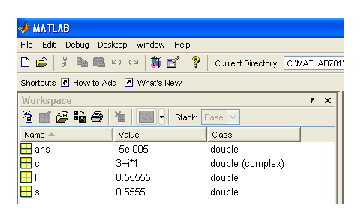
\includegraphics{NumberFormat}
    \caption{\footnotesize
            Example workspace showing floating point real and complex numbers
            \label{fig.numberformat}
            }
\end{figure}

The built-in functions listed in Table \ref{tab.complexnumfuncs} are particularly useful when dealing with complex numbers.
\begin{table}[hbt]
\begin{minipage}{\textwidth}
\centering
\begin{tabular}{c|c}
    \textit{Function}   &   \textit{Example} \\ \hline\hline
    \verb=real(c)=      &   \verb=3=        \\
    \verb=imag(c)=      &   \verb=1=        \\
    \verb=abs(c)=       &   \verb=3.1623=    \\
    \verb=angle(c)=     &   \verb=0.3218=\footnote{As with all built-in MATLAB angular functions, the default is always radians.}
\end{tabular}
\caption[Common Complex Number Functions]{\footnotesize
        Common built-in MATLAB functions dealing with complex arguments.  Here the examples use $c=3+i$.
        \label{tab.complexnumfuncs}
        }
\end{minipage}
\end{table}

\par
One must be careful because the variable names \verb=i= and \verb=j= can be reassigned by the user to be something \textit{other} than $\sqrt{-1}$.  Say, for example, that on lines 10--20 in a script there is a \verb=for= loop that uses \verb=i= as its index and runs up to \verb#i = 100#.  Then on line 25, the script tries to execute complex variable assignment \verb#x = 4+5*i;#.  Of course, unless the variable \verb=i= was cleared between lines 20 and 25, the script will create \verb#x = 504# and not the desired \verb#x = 4.0000 + 5.0000*i#.  The moral is to be very careful when using \verb=i= and \verb=j= as non-native variables.

\subsubsection{Arrays} \label{sec.matlab.array}
Arrays are the heart and soul of MATLAB (MATrix LABoratory).  Arrays are groups of numbers that travel around together.  They may be grouped so they stay in the right order, so that they perform some mathematical operation, or any other reason.  We are all familiar with one- and two-dimensional arrays.  We already know them as \textit{vectors} and \textit{matrices}, respectively.  However, MATLAB can handle higher-dimensional arrays; for these it is easier to think of every two-dimensional object as being a matrix stacked among others.
\par
Arrays are defined using square brackets: \verb=[ ]=.  Entries in a row may be separated by either a comma or whitespace (space bar).  A row is terminated and a new one begun with either a semicolon or a line break within the brackets.

\begin{codex}
>> rvec = [1 2 3 4]
rvec =
    1   2   3   4
>> cvec = [11; 12; 13; 14]
cvec =
    11
    12
    13
    14
>> TwoDimArray = [1 2 3
4 5 6
7, 8, 9]
TwoDimArray =
    1   2   3
    4   5   6
    7   8   9
\end{codex}

\par
In MATLAB, array dimensions are always listed with rows first and columns second.  For example, if we wanted to call out the 6 from the variable \verb=TwoDimArray=, we would enter

\begin{codex}
>> TwoDimArray(2,3)
ans =
    6
\end{codex}
This is because the 6 lies in the second row and the third column.  Some helpful array creation and basic modification commands are listed in Table \ref{tab.arraycreate}.
\begin{table}[bht]
\centering
\renewcommand{\arraystretch}{1.2}
\begin{tabular}{c|p{1.65in}|p{.3\textwidth}}
    \textit{Function}   &\parbox{1.5in}{\centering\textit{Description}}& \parbox{.3\textwidth}{\centering\textit{Example}} \\ \hline \hline
    \verb=ones(m,n)=    & Create an $m$ by $n$ array filled with ones &
        \verb#ones(2,3) = #$\begin{array}{ccc} 1&1&1\\1&1&1\end{array}$ \\
    \verb=zeros(m,n)=   & Same as \verb=ones=, but filled with zeros. &
        \verb#zeros(3,2)= #$\begin{array}{cc} 0&0\\0&0\\0&0\end{array}$ \\
    \verb=transpose(A)= \textit{or} \verb=A.'= & Transpose the array $A$ &
        \verb#rvec.' =#$\begin{array}{c}1\\2\\3\\4\end{array}$ \\
    \verb=size(A)=      & Return the dimensions of $A$ in an array &
        \verb#size(cvec) =#$\begin{array}{cc}4&1\end{array}$\\
    \verb=length(A)=    & Returns the maximal dimension of $A$ &
        \verb#length(rvec) =# $4$\\
    \verb=:=            & Used to span indices, ``to'' &
        \raggedright \verb#TwoDimArray(1:2,2:3)#\\ \hfill $=\begin{array}{cc}2&3\\5&6\end{array}$
\end{tabular}
\caption[Common Basic Array Functions]{\footnotesize
        Common built-in MATLAB functions useful for defining and manipulating arrays.  The examples use the variables created in Section \ref{sec.matlab.array}.
        \label{tab.arraycreate}
        }
\end{table}
\par
We can also make an array by concatenating smaller arrays.  Special attention must be paid to the dimensions in order to make a valid concatenation.

\begin{codex}
>> h = [1 2 3], k = [4; 7], m = [5 6; 8 9]
h =
    1   2   3
k =
    4
    7
m =
    5   6
    8   9
>> n = [h; k m]
n =
    1   2   3
    4   5   6
    7   8   9
\end{codex}

\par
Vectors, as we have seen, are one-dimensional examples of arrays.  To create vectors with equally spaced elements, the colon (\verb=:=) notation is helpful. The syntax is \textit{start value} : \textit{step size} : \textit{end value}.  The default step size is $1$.

\begin{codex}
>> c = 2:5, d = 9:-1:3
c =
    2   3   4   5
d =
    9   8   7   6   5   4   3
\end{codex}
A useful trick is to use a vector to call indices from another vector.  For example, using the above variable \verb=c=, we can call the second through the fifth values from \verb=d= in the following way:

\begin{codex}
>> d(c)
ans =
    8   7   6   5
\end{codex}

\par
The following are more complex examples of arrays and indices.

\begin{codex}
>> m = [1.5 -2.4 3.5 0.7; -6.2 3.1 -5.5 4.1; 1.1 2.2 -0.1 0]
m =
    1.5     -2.4    3.5     0.7
    -6.2    3.1     -5.5    4.1
    1.1     2.2     -0.1    0
>> n = m(1:2,2:4), o = m(:,1:2), p = m(2,:)
n =
    -2.4    3.5     0.7
    3.1     -5.5    4.1
o =
    1.5     -2.4
    -6.2    3.1
    1.1     2.2
p =
    -6.2    3.1     -5.5    4.1
\end{codex}

\subsubsection{Strings} \label{sec.matlab.string}
Strings (or sometimes character strings) are very much like vectors.  The difference is that the entries are characters instead of numbers.  Strings are defined by single quotation marks.

\begin{codex}
>> str = 'Signal and System Analysis';
>> disp(str)
Signals and System Analysis
>> str(1:6)
Signal
\end{codex}

\par
Strings are useful when we wish to load several files that have been given sequential names (like \textit{data1.dat}, \textit{data2.dat}, etc.).  In this case, a \verb=for= loop may be created that executes commands on the string \verb=data= concatenated with the index 1, 2, etc.

\subsubsection{Logicals}
When MATLAB performs a logical operation (see Section \ref{app.oper.logic}), the output is always binary in nature.  That is, the output is an array of 1's and 0's.  This output is then dual-purpose:  It contains numbers in indexed positions (like arrays) but it also contains ``true/false'' values in indexed positions.  In this sense, logical arrays are very handy because they serve dual purposes and may be processed very quickly.
\par
There is a key difference between arrays and logicals regarding indexing.  When using an array to call the index, the value of the elements of the array is important.  When using logicals, only the position of the ``true'' elements is important.

\begin{codex}
>> a = 2:1:5, b = a>3
a =
    2   3   4   5
b =
    0   0   1   1
>> a(b)
ans =
    4   5
>> a([3:4])
ans =
    4   5
>> notlogical = [0 0 1 1];
>> a(notlogical)
??? Subscript indices must either be real positive integers
    or logicals.
\end{codex}

\par
The last line is an error because MATLAB thinks we are looking to create an array with the first two elements being the $0^{th}$ element of \verb=a= and the third and fourth elements as the $1^{st}$ element of \verb=a=.  When MATLAB looks for the $0^{th}$ element of \verb=a=, it gets confused because indices can only be positive integers ($1,2,3,\ldots$).

\subsubsection{Cells}
Cells are convenient ways to store objects of several different types.  They are created and their indices are called with \{curly braces\} and act very much like arrays.  However, a one-dimensional cell may have an entire matrix at position 1 but a single character at position 2.  Cells do not have a clear analog like arrays do to matrices, so it may be more convenient to simply think of them as ``multimedia'' arrays.

\begin{codex}
>>  M = [1 2; 3 4];
>>  str = 'This is my matrix';
>>  cell1 = {M str}
cell1 =
    [2x2 double]    'This is my matrix'
>> cell1{1}
ans =
    1   2
    3   4
>>
\end{codex}

\subsubsection{Special Numbers}
In addition to the imaginary numbers \verb=i= and \verb=j=, MATLAB has two other special predefined variables.  They are \verb=pi= and \verb=Inf=.  The variable \verb=pi= is MATLAB's closest estimate at the irrational number $\pi$.  The variable \verb=Inf= represents infinity and results from actions like dividing by zero or that result in a number larger than MATLAB can handle.
\par
Furthermore, operations like $\frac{0}{0}$ and $\sin \infty$ produce undefined results and are represented by \verb=NaN=, which stands for ``not a number.''

\section{Operations}
The operations in the above sections have been minimal and intuitive.  Here we look at some of the more advanced operations MATLAB can perform.

\subsection{Arithmetic Operations} \label{sec.matlab.arithop}
MATLAB defines all arithmetic operations in matrix terms.  Note that a single number may be either a scalar or a one-by-one matrix, but its operations are all treated as matrix ones.  Issuing \verb=help arith= and \verb=help slash= will list the available arithmetic operations.
\par As one would expect, the \textit{order} of operations is often important. We have seen that MATLAB executes commands from left to right.  However, within a command, MATLAB follows the familiar \textit{PEMDAS} (parentheses, exponents, multiplication and division, then addition and subtraction) order.
\par
It is also important to observe that the operators ``slash'' \verb=/= and ``backslash'' \verb=\= represent two different matrix operations.  For example, \verb=B/A= is right division and represents $BA^{-1}$ whereas \verb=A\B= is left division and represents $A^{-1}B$.  We know that these may be two \textit{very} different quantities, so it is important to differentiate between them.

\begin{codex}
>> a = [1 2; 3 4]; b = [3 1; 7 8]; c = [2 4];
>> d = a + b, e = c*a, f = a^2, g = c'
d =
    4   3
    10  12
e =
    14  20
f =
    7   10
    15  22
g =
    2
    4
>> h = a\b, k = b/a
h =
    1.0000  6.0000
    1.0000  -2.5000
k =
    -4.5000 2.5000
    -2.000  3.0000
\end{codex}

\par
To use an operator on an element-by-element basis rather than its matrix math sense, use the modifier of a period (\verb=.=) prior to the operator.  This tells MATLAB to perform the operation among entries with the same location in their respective arrays.

\begin{codex}
>> m = a.*b, n= b./a, o = b.^a
m =
    3   2
    21  32
n =
    3.0000  0.5000
    2.3333  2.0000
o =
    3   1
    343 4096
\end{codex}

\subsection{Logical Operators} \label{app.oper.logic}
The logical operations AND, OR, and NOT are specified by ampersand (\verb=&=), pipe (\verb=|=), and tilde (\verb=~=) respectively.  They can be used in conjunction with the relation operators listed in Table \nolinebreak[3] \ref{tab.relationoperations} to construct logical arrays as in the examples below.  As usual, ``true'' is represented by 1 and ``false'' by 0.

\begin{table}[bht]
\centering
\begin{tabular}{c|c}
    \textit{Relation}       &   \textit{Symbol} \\ \hline \hline
    Less than               &   \verb#<# \\
    Less than or equal to   &   \verb#<=# \\
    Greater than            &   \verb#># \\
    Greater than or equal to&   \verb#>=# \\
    Equals exactly          &   \verb#==# \\
    Does not equal          &   \verb#~=#
\end{tabular}
\caption[Relation Operations]{\footnotesize
        Relation operator symbols
        \label{tab.relationoperations}
        }
\end{table}

\begin{codex}
>> a = [1 3 2; 4 6 5], b = a>2 & a<=5
a =
    1   3   2
    4   6   5
b =
    0   1   0
    1   0   1
>> c = [1 5 3 4 7 8], d = c>4
c =
    1   5   3   4   7   8
d =
    0   1   0   0   1   1
\end{codex}

\par
Further, logical arithmetic operations may be mixed in a single command.  Priority is given to the arithmetic operations first, however.

\begin{codex}
>> 5 + 2 > 6 * 8
ans =
    0
>> 5 + 2 > 6
ans =
    1
>> 5 + (2>6) * 8
ans =
    5
\end{codex}

\subsection{Mathematical Operations} \label{sec.matlab.mathop}
Another of MATLAB's strengths is its vast library of built-in mathematical functions.  These range from utterly simple to quite complicated.  A sampling of commonly useful math operations is listed in Tables \ref{tab.mathoperations} and \ref{tab.trigfunctions}.

\begin{table}[bht]
\centering
\subfloat[Commonly used built-in mathematical functions \label{tab.mathoperations}]{
\renewcommand{\arraystretch}{1.2}
\begin{tabular}{c|c}
    \textit{Command}&   \textit{Description} \\ \hline \hline
    \texttt{exp(x)}   & Base $e$ exponent of $x$ \\
    \texttt{log(x)}   & Base $e$ logarithm of $x$ \\
    \texttt{log10(x)} & Base $10$ logarithm of $x$ \\
    \texttt{complex(a,b)}& Construct the complex number $a+bi$ \\
    \texttt{conj(x)}  & Complex conjugate of $x$ \\
    \texttt{round(x)} & Round $x$ to the nearest integer \\
    \texttt{floor(x)}& Round $x$ toward $-\infty$ \\
    \texttt{ceil(x)}  & Round $x$ toward $\infty$
    \end{tabular}
    }\\
\vspace{0.75cm}
\subfloat[Commonly used built-in trigonometry functions \label{tab.trigfunctions}]{
\renewcommand{\arraystretch}{1.2}
\begin{tabular}{c|c}
    \textit{Command}&   \textit{Description} \\ \hline \hline
    \texttt{sin(x)}   & $\sin x$ \\
    \texttt{cos(x)}   & $\cos x$ \\
    \texttt{tan(x)}  & $\tan x$ \\
    \texttt{asin(x)}  & $\arcsin x$ \\
    \texttt{acos(x)}    & $\arccos x$ \\
    \texttt{atan(x)}    & $\arctan x$ \\
    \texttt{atan2(y,x)}   & \parbox{1.5in}{\centering $\arctan (yi+x)$\\ Restricted to $-\pi$ to $\pi$}
\end{tabular}
}
\caption{}
\end{table}

\subsection{Data Analysis Operations} \label{sec.matlab.dataana}
One may use MATLAB to perform analysis on sets of data collected elsewhere.  There are several built-in MATLAB functions that calculate certain statistics or ease the process of data analysis.  Table \ref{tab.dataanalysis} contains a sample of these.

\begin{table}[bht]
\centering
\renewcommand{\arraystretch}{1.2}
\begin{tabular}{c|p{1.65in}|p{.3\textwidth}}
    \textit{Function}   &\parbox{1.5in}{\centering\textit{Description}}& \parbox{.3\textwidth}{\centering\textit{Example}} \\ \hline \hline
    \verb=find(a)=  & Returns indices of nonzero elements &
        \verb#find(a) = #$\begin{array}{cccc}1&3&4&6\end{array}$ \\
    \verb=find(a>b)= & Returns indices for which logical expression is true&
        \verb#find(a>2) = #$\begin{array}{cc}4&6\end{array}$    \\
    \verb=max(a,[],d)= & Returns the maximum elements along the direction
        specified & \verb#max(a) = #$4$ \\
    \verb=min(a,[],d)= & Returns the minimum elements along the direction
        specified & \verb#min(a) = #$0$ \\
    \verb=mean(a,d)= & The average of the elements &
        \verb#mean(a) = #$1.6667$ \\
    \verb=sum(a,d)= & The sum of the elements   &
        \verb#sum(a) = #$10$
\end{tabular}
\caption{\footnotesize
        Commonly used data analysis functions.
        All relevant examples operate on the vector
        $a = (1,0,2,3,0,4)$.
        The optional arguments \texttt{[],d} can be used to specify the dimension on which the function is to act.  In all cases
        \texttt{d = 1}
        operates on columns and returns a row, and
        \texttt{d = 2}
        is the opposite.
        \label{tab.dataanalysis}
        }
\end{table}

\section{Flow Control} \label{sec.matlab.flowcont}
Like many other programming languages, MATLAB uses flow control statements to repetitively or selectively execute statements.  Once activated, all statements are executed until the \verb=end= command.

\subsection{\texttt{for} Statement}
The \verb=for= statement executes commands a fixed number of times.  It is equivalent to the \verb=do= command found in other languages.  For example, to evaluate the summation
\begin{equation*}
    x(t) = \sum_{k=1}^{3} t^{\sqrt{1.2k}} \sqrt{k}
\end{equation*}
for times between 0 and 0.8 seconds at intervals of 0.2 seconds, we would execute:

\begin{codex}
t = 0 : 0.2 : 0.8;
x = zeros(size(t));
for k = 1 : 3
    x = x + sqrt(k)*t.^sqrt(1.2*k);
end

>>  x
x =
    0   0.3701  1.0130  1.8695  2.9182
\end{codex}
In the above example, we \textit{initialized} the variable \verb=x= to be all zeros before we executed the \verb=for= loop.  This is good programming practice because in larger or nested loops, it is faster for the system to assign values to already existing elements, rather than resize the variable on every iteration.
\par
\textit{Nested} \verb=for= loops involve executing entire sub-loops on every iteration of outer loops.  In the example below, \verb=m= starts at 1, and \verb=n= runs from 1 to 4 before \verb=m= advances to 2; Then the process repeats.

\begin{codex}
y = zeros(3,4);
for m = 1 : 3
    for n = 1 : 4
        y(m,n) = m + n;
    end
end

>>  y
y =
    2   3   4   5
    3   4   5   6
    4   5   6   7
\end{codex}
It is often important to remember to place the semicolon after each line inside of the loops.  If omitted, MATLAB will display that line every time it is iterated.  This can significantly slow the execution time of a script.

\subsection{\texttt{while} Statement}
The \verb=while= statement is similar to the \verb=for= statement except that the loop terminates when a logical condition is satisfied.  To find the largest power of 2 that is less than 5,000, we might use

\begin{codex}
n = 1;
while n*2 < 5000
    n = n*2;
end

>>  n
n =
    4096
\end{codex}
Care should be taken when using \verb=while= loops because there is a possibility that poorly stated logical conditions may never be satisfied; this results in an endless loop.\\[6pt]
\parbox{\textwidth}{\mbox{\large \uline{Important}:} Should you find yourself in an infinite loop, press Control-c in the Command Window to terminate the current process.}
\vspace{1pt}
\par
Another common use of \verb=while= statements is to perform tasks while a certain variable counts down towards zero.  Here it is appropriate to introduce a concept called ``machine zero.''  MATLAB systems have a least counting element, it is the smallest quantity that the system can differentiate between numbers.  On most modern installations, it is around $10^{-16}$.  So if a \verb=while= loop is set to run until the counter reaches zero, it will actually run until the counter reaches $\pm 10^{-16}$.
\par
This may be a problem if the counter only asymptotically approaches zero.  It may take many iterations to reach the machine zero.  In this case, it is useful to define a number that is ``close enough'' to zero for the loop to terminate. This value, called the stopping point, represents a trade-off between absolute accuracy and execution speed.

\subsection{\texttt{if} Statement}
The \verb=if= statement allows us to selectively execute statements based on the outcome of a logical expression.  Further, they can be nested within other loops as well as other \verb=if= statements.

\begin{codex}
for k = 1 : 4
    if k == 1
        x(k) = 3*k;
    else
        if k == 2 | k == 4
            x(k) = k/2;
        else
            x(k) = 2*k;
        end
    end
end

>>  x
x =
    3   1   6   2
\end{codex}
In addition, \verb=if= statements are often used to issue warnings or check for data errors before performing intense calculations.

\begin{codex}
c = 't'; n = 2;
if c == 'f'
    c = 'false'
    y = NaN;
end
d = 0.1 : 0.1 : 0.4;
if c == 't'
    if n == 2
        y = 100*d(n);
    elseif n == 1
        y = 10*d(n);
    else
        y = 0;
    end
end
\end{codex}
Which of course yields \verb#c = t# and \verb#y = 20#.
\par
When used with \verb=if= statements, the \verb=break= command is very useful.  If a loop is to be executed a variable number of times, \verb=if= statements can be used to check the status of certain criteria, and then the \verb=break= command can be issued to halt the loop.

\section{Plotting}
Plotting---in two dimensions or three---is an extremely useful tool in the analysis and presentation of data.  Even if they are never destined to be published, plots often give a ``big picture'' idea of a data set that is more valuable than numerical or statistical analysis alone.
\par
As such, MATLAB has a wealth of graphical display functions from the urbane to the imaginative.  The most basic is the \verb=plot(x,y)= command.  This places a connected plot of the data pairs $x(k),y(k)$ for all $k$ in the current figure window.  The following three lines of code generate the plot in Figure \ref{fig.matlab.plainplot}.

\begin{codex}
x = linspace(0, 2*pi);
y = sin(x);
plot(x,y);
\end{codex}

\begin{figure}[hbp!]
\centering
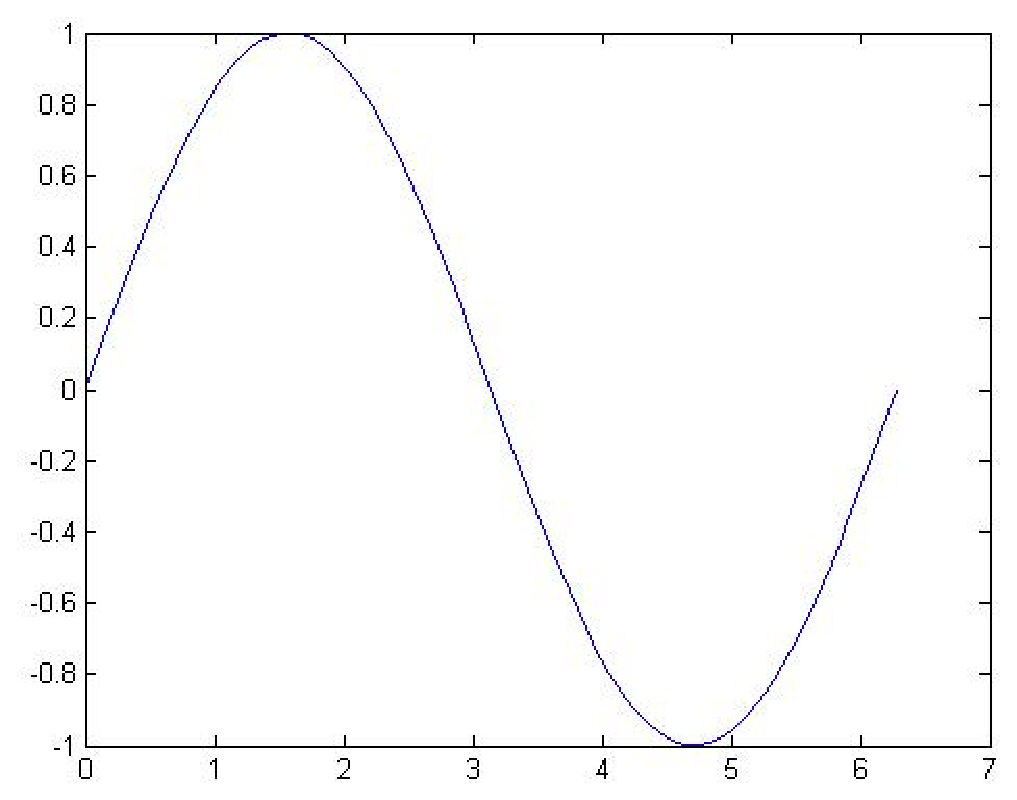
\includegraphics[width=.9\textwidth]{plainplot}
\caption{\footnotesize
        Simple plot generated from three lines of code.
        \label{fig.matlab.plainplot}
        }
\end{figure}

Of course, the plot in Fig.~\ref{fig.matlab.plainplot} is presentable and the ease with which it was generated is nice.  But it is lacking somewhat in presentation (what are we looking at?) and functionality (why are we looking at it?).  As such, MATLAB provides many more commands to create detailed graphs and dress them up nicely.
\par
In particular, the \verb=plot= command itself has many optional arguments.  Issuing \verb=help plot= details all of the different line and marker styles available.

\begin{table}[hbp!]
\begin{minipage}{\textwidth}
\centering
\renewcommand{\arraystretch}{1.3}
\begin{tabular}{c|p{0.55\textwidth}}
    \textit{Command}& \multicolumn{1}{c}{\textit{Description}}\\ \hline \hline
    \verb=figure(a)=    &   Makes \verb=a= the active figure window\\
    \verb=hold on=      &   Places subsequent plot commands on same axes instead of replacing them \\
    \verb=hold off=     &   Releases \verb=hold on= command\\
    \verb=title(`text')=&   Places \verb=text= as a title above the plot\\
    \verb=xlabel(`text')=&  Labels x-axis of plot with \verb=text=\\
    \verb=ylabel(`text')=&  Labels y-axis of plot with vertically rotated
                                \verb=text=.\\
    \verb=text(x,y,`text')=& Places \verb=text= on the plot at point $(x,y)$\\
    \verb=legend('First','Second')= & Places a legend that labels two plots on the same axes\\
    \verb=axis([x1 x2 y1 y2])=      & Scales the x- and y-axes to fit between $x_1$, $x_2$, $y_1$, and $y_2$\\
    \verb=subplot(m,n,id)=& Splits the figure window into an $m$ by $n$ array of plots with plot number \verb=id= as the active plot\footnote{In a \texttt{subplot} array, the plots are numbered starting at 1 in the upper left and count across the first line, then across the second line, etc.}
    \end{tabular}
\caption{\footnotesize
        Common plot editing commands
        \label{tab.plotting}
        }
\end{minipage}
\end{table}

We now expand on the three-line example above to incorporate some of the commands detailed in Table \ref{tab.plotting}.  The resulting graph is shown in Figure \ref{fig.matlab.fancyplot}.

\begin{codex}
x = linspace(0, 2*pi);
y1 = sin(x);
y2 = cos(x);
ax = [0 2*pi -1.5 1.5];
figure;
subplot(2,1,1)
plot(x,y1,'o')
axis(ax)
title('Basic Sinusoids')
ylabel('y-axis')
legend('Sin(x)')
subplot(2,1,2)
plot(x,y2,'+-')
axis(ax)
xlabel('x-axis')
ylabel('y-axis')
legend('Cos(x)')
\end{codex}

\begin{figure}[hbp!]
\centering
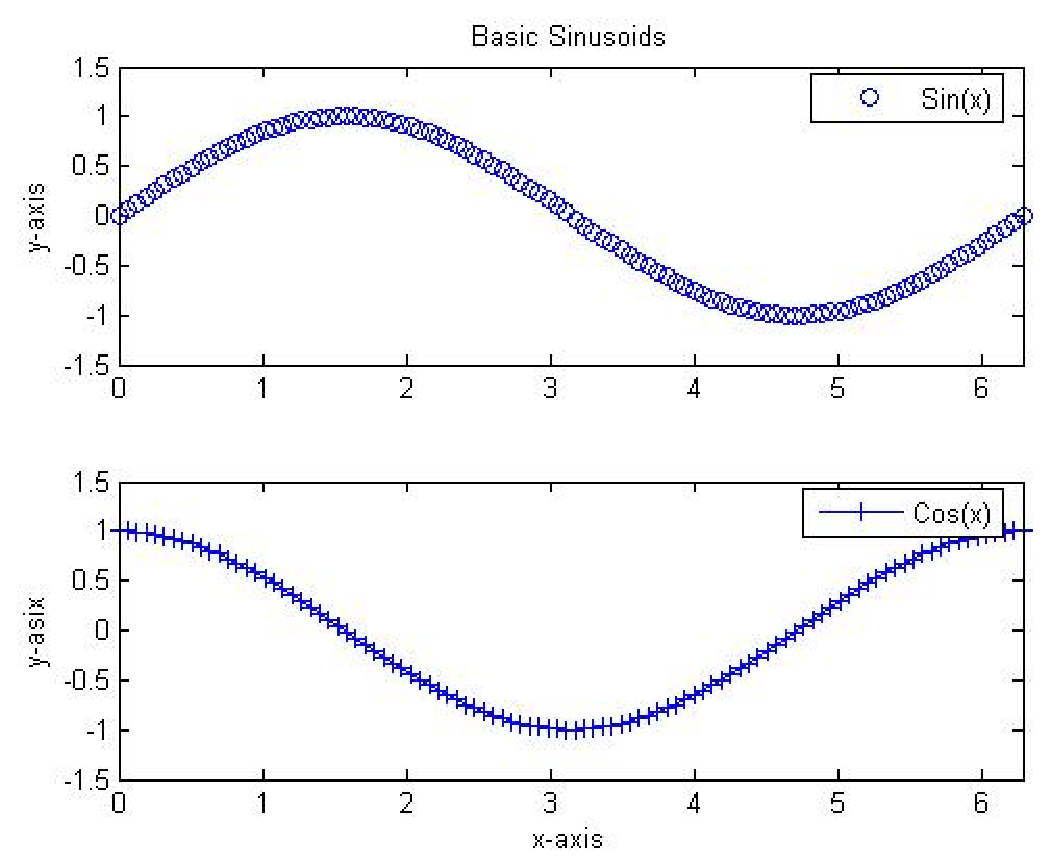
\includegraphics[width=0.9\textwidth]{fancyplot}
\caption{\footnotesize
        Embellished plots using tools from Table \ref{tab.plotting}
        \label{fig.matlab.fancyplot}
        }
\end{figure}

\section[Signals and Systems Applications]{Signals and Systems Applications\footnote{Section \ref{sec.matlab.sigsys} is taken directly from the first edition of this laboratory manual.  It's author is unknown.} \label{sec.matlab.sigsys}
}
In this section, we present several function m-files that have been created specifically for signal and system analysis.  On the laboratory com\-puters, these m-files are loc\-ated in
\begin{verbatim}
w:\matlab\toolbox\ee351L
\end{verbatim}
These functions encompass
\begin{itemize}
    \item Step and ramp signal functions
    \item Discrete- and continuous-time Fourier series functions
    \item Continuous-time Fourier transform function
\end{itemize}
All of the functions contain help statements at the beginning.  These statements indicate the function's purpose, define input and output variables, and in a  few cases provide useful modification suggestions and requirements.

\subsection{Step and Ramp Functions}
We use step and ramp functions often in signal and system analysis.  Therefore, we have created the MATLAB functions \verb=us= and \verb=ur= to compute them.  The syntax looks like
\begin{verbatim}
u = us(t)
r = ur(t)
\end{verbatim}
The step function \verb=us= returns $u=0$ for $t<0$ and $u=1$ for $t\geq0$.  Likewise, \verb=ur= returns $r=0$ for $t<0$ and $r=t$ for $t\geq 0$.

\subsection{Continuous-Time Fourier Series Functions}
We have created four functions for use in performing Fourier analyses of continuous-time signals.  The first function computes Fourier series coefficients from sample values of a continuous-time signal.  The second function computes samples of the truncated Fourier series approximation to a signal over a specified time interval.  The last two functions compute the Fourier transform and the inverse Fourier transform, respectively.

\subsubsection{Fourier Series Coefficients}
The function
\begin{verbatim}
[Xn, f, ang, No, Fo] = ctfsc(t,x)
\end{verbatim}
computes the Fourier series expansion coefficients \verb=Xn= corresponding to the portion of the signal \verb=x= within the expansion interval \verb=t(1) - dt/2= to \verb=t(ns) + dt/2=.  This interval has length \verb=ns*dt= where \verb#ns = size(t,2)# is the number of signal samples and \verb=dt= is the time interval between samples.
\par
There are \verb=ns= Fourier series coefficients computed and the frequency interval between these is \verb#Fo = 1/(ns*dt)#.  Series coefficients are computed for both positive and negative frequencies and the coefficient $X_0$ corresponding to $f = 0$ is stored in \verb=Xn(No)=.  The values of both \verb=No= and \verb=Fo= are function outputs along with \verb=Xn=.
\par
The Fourier series expansion interval can begin anywhere between \verb=-10*(ns*dt)= to \verb=10*(ns*dt)=.  These limits can be changed, if required, as indicated in the help statements in the m-file.

\subsubsection{Truncated Fourier Series}
The second Fourier series function is
\begin{verbatim}
[xfs, Xnn] = ctfs(t,Xn,no,fo,N)
\end{verbatim}
This function first selects the \verb=2N+1= Fourier series coefficients, \verb=Xnn=, centered on $X_0$.  Then the function computes samples, \verb=xfs=, of the truncated Fourier series approximation of $x$ over the time interval specified by the input variable \verb=t=.  The time interval does not need to be the same as the expansion interval used to compute the Fourier series coefficients.
\par
The input variables \verb=Xn=, \verb=no=, and \verb=fo= are the output variables obtained from the function \verb=ctfsc=.  This function also plots the Fourier series.  The original function can also be plotted on the same graph by using the \verb=hold on= command after \verb=ctfs= followed by the \verb=plot= command.

\subsubsection{Fourier Transform}
MATLAB contains  a built-in function for the Fourier transform called \verb=fft=.  Using this function requires knowledge of discrete-time concepts which students in this laboratory are not expected to know.  We have therefore written a function which attempts to create the best approximation possible to a continuous-time Fourier transform.
\par
The function
\begin{verbatim}
[f, X, N, no] = ctft(t,x,dfm)
\end{verbatim}
computes the Fourier transform of the portion of the signal \verb=x= contained in the interval \verb=t(1) - dt/2= to \verb=t(ns) + dt/2=.  This interval has length \verb=ns*dt= where \verb#ns = size(x,2)# is the number of signal samples and \verb=dt= is the time interval between samples.  The signal portion used must begin at \verb=t(1)$\leq 0$ and end at \verb=t(ns)= $>0$.  If the signal is longer than the time interval \verb=ns*dt=, then the computed transform will have some distortion since it is the transform of the truncated signal.
\par
There are \verb=N= Fourier transform samples computed, where \verb=N= is the larger of \linebreak[4] \verb=ceil( 1/(dfm*dt) )= or \verb=2*ns=.  The variable \verb=dfm= is the maximum spacing that we will allow between computed transform samples.  Note that care must be exercised in selecting \verb=dfm= and \verb=dt= since \verb=N= can become very large if they are chosen to be quite small.  Transform samples are computed for both positive and negative frequencies with a spacing of \verb#df = 1/(N*dt)#.  The transform value at $f=0$ is stored in \verb=X(no)=.  The frequencies at the transform sample points are stored in the output vector \verb=f=.
\par
Now we can plot the magnitude and phase of the Fourier transform using MATLAB's plot capabilities.  We can use the \verb=subplot= command to plot the amplitude and angle of the transform on the same page:

\begin{codex}
subplot(2,1,1)
plot(f,abs(X))
subplot(2,1,2)
plot(f,angle(X))
\end{codex}

\par
Due to complications arising from the fact that we are actually using discrete-time signals in our computations, the phase of the Fourier transform may sometimes be different from what is expected.  If this happens, first try using the \verb=unwrap= command before plotting the phase.  If the problem still exists, the problem may be that an insufficient portion of the signal is begin included in the samples.  Try extending the length of the samples in include a longer portion of the signal.

\subsubsection{Inverse Fourier Transform}
MATLAB contains a built-in function for the inverse Fourier transform called \verb=ifft=.  Using this function requires knowledge of discrete-time concepts which students in this laboratory are not expected to know.  We have therefore written a function which attempts to create the best approximation possible to a continuous-time inverse Fourier transform.
\par
The function
\begin{verbatim}
[t, x, n] = ctift(f,X,dtm)
\end{verbatim}
computes the inverse, \verb=x=, of the Fourier transform \verb=X=.  The input vector \verb=f= specifies the frequency interval and sample spacing for the input Fourier transform vector \verb=X=.  These input vectors are outputs of the function \verb=ctft=.  The number of transform samples is \verb#ns = size(X,2)#, and the number of inverse transform samples computed, \verb=N=, is the larger of \verb=ceil( 1/(dtm*df) )= or \verb=ns=.  The variable \verb=df= is the spacing between transform samples, and the input variable \verb=dtm= specifies the maximum spacing that we allow between computed inverse transform samples.  As for the Fourier transform, we must exercise care in selecting the variables \verb=df= and \verb=dtm= so that \verb=N= does not become excessively large.
\par
If the magnitude of the transform is an even function of frequency and the phase of the transform is an odd function of frequency, then the inverse transform should be real.  There will probably be some round-off error present, so in this case you should probably take the real portion of the inverse transform before plotting.  The inverse transform can then be plotted using the standard MATLAB plot command:

\begin{codex}
x = real(x);
plot(t,x)
\end{codex}

\subsection{Straight-Line Approximate Bode Plot Functions}
Straight-line approximations to Bode amplitude response and Bode phase response plots are convenient in continuous-time system analyses.  We have created the two functions \verb=sysdat= and \verb=slbode= to compute the parameters for the straight-line approximations and the straight-line approximation data, respectively.  The location of the system zeros is not restricted.  The functions are capable of finding the parameters and straight-line date for causal, stable systems (poles only in the LHP) and non-causal, stable systems (poles in both the LHP and RHP).  Also, results for marginally stable systems can be obtained.  These results are valid for input signals that do not contain poles located at single-order system poles on the imaginary axis.

\subsubsection{Transfer Function Parameter Computation}
The function
\begin{verbatim}
[rn, rd, imas, rhps, c, bf, ft, dr] = sysdat(n,d)
\end{verbatim}
computes the transfer function, or frequency response, parameters for a system having the transfer function
\begin{equation*}
    H(s) = \frac{n(1)s^\alpha + \cdots + n(\alpha)s + n(\alpha+1)}{
        d(1)s^\beta + \cdots + d(\beta)s + d(\beta+1)}
\end{equation*}
or frequency response
\begin{equation*}
    H(j\omega) = \frac{n(1)(j\omega)^\alpha + \cdots + n(\alpha)j\omega +
        n(\alpha+1)}{d(1)(j\omega)^\beta + \cdots + d(\beta)j\omega +
        d(\beta+1)}
\end{equation*}
The numerator and the denominator coefficients are stored int he input vectors \verb=n= and \verb=d=, respectively.  Function outputs are described in Table \ref{tab.matlab.transfunccomp}.

\begin{table}[bht]
\centering
\renewcommand{\arraystretch}{1.3}
\begin{tabular}{c | p{0.65\textwidth}}
    \textit{Output Variable}& \multicolumn{1}{c}{\textit{Description}}\\ \hline \hline
    \texttt{rn}     &   Roots of the numerator (system zeros) \\
    \texttt{rd}     &   Roots of the denominator (system poles) \\
    \texttt{imas}   &   Two-element row vector containing the number of zeros
                        and the number of poles on the imaginary axis   \\
    \texttt{rhps}   &   Two-element row vector containing the number of zeros
                        and the number of poles in the RHP  \\
    \texttt{c}      &   Constant multiplicative factor $c=n(i)/d(j)$,
                        where $i$ and $j$ are the largest integers for which $n(i)$ and $d(j)$ are not equal to zero \\
    \texttt{bf}     &   Row vector containing the break frequency for each
                        factor where, for linear factors \texttt{bf}$>0$, \texttt{bf}$=0$, and \texttt{bf}$>0$ indicate LHP, imaginary axis, and RHP poles or zeros, respectively\\
    \texttt{ft}     &   Row vector of factor types where $+1$ and $+2$
                        correspond to numerator linear and quadratic factors, and $-1$ and $-2$ correspond to denominator linear and quadratic factors   \\
    \texttt{dr}     &   Row vector of factor damping ratios
\end{tabular}
\caption{\footnotesize
        Output argument descriptions for the custom function \texttt{sysdat}.
        \label{tab.matlab.transfunccomp}
        }
\end{table}

\par
A damping ratio only applies to a quadratic factor and is a number greater than zero but less than one.  We set \verb=dr(i)= equal to $10$ for factor \verb=i= as an indicator that factor \verb=i= is a linear factor.  Quadratic factors that correspond to LHP, imaginary axis, and RHP poles are indicated with positive, zero, and negative damping ratios, respectively.
\par
\uline{Note}: If a factor is of order $N$, then the data for it will appear as data for $N$ first order factors at the same break frequency.  The data for each of these first-order factors is the same and the resulting straight-line approximation for the $N^{th}$-order factor is the sum of the straight-line approximations for the $N$ first-order factors.

\subsubsection{Straight-Line Data Computation}
We compute the straight-line Bode plot approximation data with the function
\begin{verbatim}
[am, ph] = slbode(w,c,bf,ft,dr)
\end{verbatim}
The input variables include the vector \verb=w= defining the frequency interval and increment for which the data are computed.  The other input variables are the frequency  response factor parameters computed with function \verb=sysdat=.  These are defined in Table \ref{tab.matlab.transfunccomp}.
\par
The output variables are the vectors \verb=am= and \verb=ph=.  These contain the data for the straight-line approximations to the amplitude-response and phase-response Bode plots, respectively.

\begin{thebibliography}{9}
    \bibitem{chapman} Stephen J. Chapman. MATLAB Programming for Engineers, 2nd edition.  Thomson Engineering, 2001
    \bibitem{mathworks} Mathworks website.  http://www.mathworks.com/
    \bibitem{firsted} EE351L Laboratory Manual, 1st edition.
\end{thebibliography}